% !TEX root = presentation.tex
\section{Approach}
\subsection{Thesis Statement}
\frame{\frametitle{Thesis Statement}
  \begin{large}
    \textit{``The use of source code and test suite \alert{metrics} in combination with \alert{machine learning} techniques can accurately predict \alert{mutation scores}. Furthermore, the predictions can be used to \alert{reduce} the performance \alert{cost} of mutation testing when used to iteratively develop test suites.''}
  \end{large}
  \vspace{5mm}
  \hrule
  \vspace{5mm}
  \begin{itemize}
    \item A \alert{``do fewer and smarter''} technique for mutation testing.
    \begin{itemize}
      \item Identify source code units that have \alert{low/high coverage}.
      \item Ability to \alert{prioritize} mutation testing for specific mutants.
    \end{itemize}
  \end{itemize}
}

\subsection{Process}
\frame{\frametitle{Process}
  \begin{enumerate}
    \item Data collection.
    \item Data synthesis.
    \item Data prediction.
  \end{enumerate}
}

\subsubsection{Data Collection}
\frame{\frametitle{Data Collection}
  \begin{columns}
    \begin{column}{5.75cm}
      \flushleft
      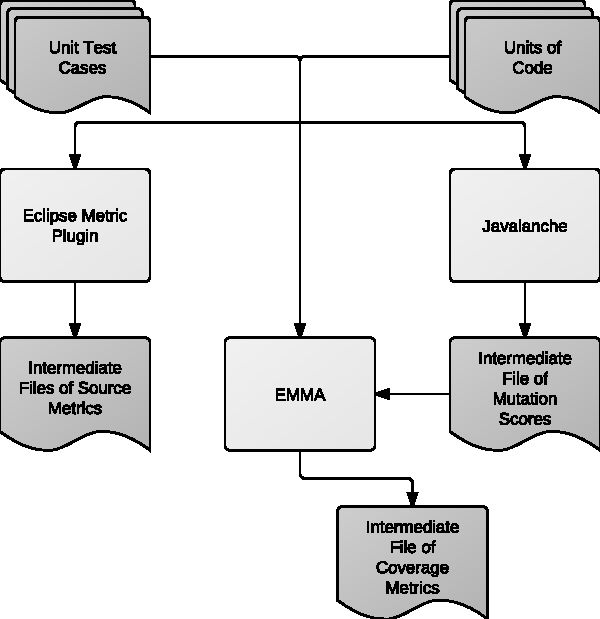
\includegraphics[width=5.25cm]{../thesis/figures/process_a_clean.pdf}
      \vspace{-4mm}
      \Huge \centering
      \ldots
    \end{column}
    \qquad
    \begin{column}{5.75cm}
      \begin{itemize}
        \item \textbf{Input} -- Units of \alert{test cases} and units of \alert{source code}:
        \begin{enumerate}
          \item Collect \alert{mutation scores} using \textit{Javalanche}\footnote{\tiny{\url{github.com/david-schuler/javalanche}}}.
          \item Collect \alert{source code} metrics using \textit{Eclipse Metrics Plugin}\footnote{\tiny{\url{metrics2.sourceforge.net/}}}.
          \item Collect \alert{coverage} metrics using \textit{EMMA}\footnote{\tiny{\url{emma.sourceforge.net/}}}.
        \end{enumerate}
      \end{itemize}
    \end{column}
  \end{columns}
}

\subsubsection{Data Synthesis}
\frame{\frametitle{Data Synthesis}
  \begin{columns}
    \begin{column}{5.75cm}
      \Huge \centering
      \ldots
      \vspace{-2mm}
      \flushleft
      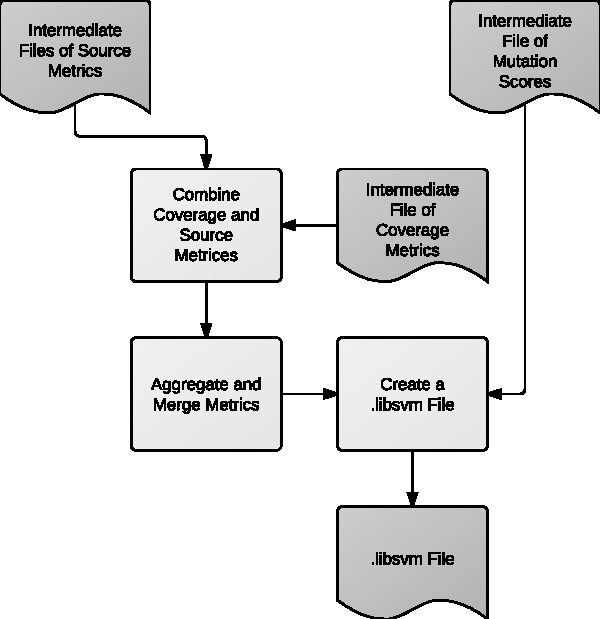
\includegraphics[width=5.25cm]{../thesis/figures/process_b_clean.pdf}
    \end{column}
    \qquad
    \begin{column}{5.75cm}
      \begin{itemize}
        \item \textbf{Output} -- \alert{Category/feature data} for source code units:
        \begin{enumerate}
          \item \alert{Combine} source code and coverage metrics together.
          \item \alert{Merge} source code metrics of the touched tests for each source code unit.
          \item \alert{Aggregate} method-level source code unit metrics into class-level source code units.
          \item \alert{Create} \texttt{.libsvm} file using feature/category data.
        \end{enumerate}
      \end{itemize}
    \end{column}
  \end{columns}
}

\subsubsection{Data Prediction}
\frame{\frametitle{Data Prediction}
  \begin{columns}
    \begin{column}{4.75cm}
      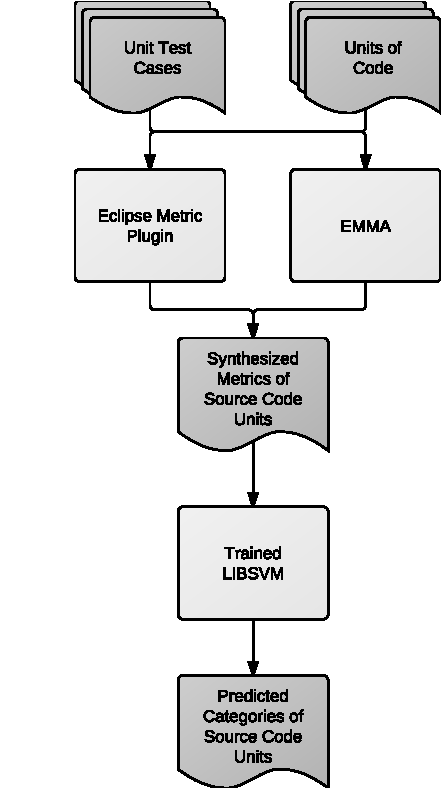
\includegraphics[width=4cm]{../thesis/figures/process_prediction_clean.pdf}
    \end{column}
    \qquad
    \begin{column}{6.75cm}
      \begin{itemize}
        \item \textbf{Predict} -- Use \alert{trained} support vector machine.
        \begin{enumerate}
          \item \alert{Collect} source code and test suite metrics.
          \item \alert{Synthesis} collected metrics.
          \item Use \alert{trained} LIBSVM\footnote{\tiny{\url{csie.ntu.edu.tw/~cjlin/libsvm/}}} to make \alert{prediction} for source code units.
        \end{enumerate}
      \end{itemize}
    \end{column}
  \end{columns}
}

\subsection{Related Work}
\frame{\frametitle{Related Work}
  \begin{itemize}
    \item Analysis of \alert{test effectiveness and coverage}~\footcite{Ino12}.
    \item \alert{Bug prediction and localization}:
    \begin{itemize}
      \item Using source code~\footcite{MKPS00}.
      \item Using bug reports~\footcite{KL05}.
      \item Using test coverage~\footcite{WDC10}.
    \end{itemize}
  \end{itemize}
}
